\anothertitle{Questions}{}


% Title, image and subtitle
\titleimage{Title and graphics}{Description of picture.}{archDiagram}

% Two-column with image 
\begin{frame}
    \Frametitle{Two-column layout with graphics}
    Normal text.

    \begin{columns}
        \column{0.5\textwidth}
        \begin{itemize}
        \item Bullet
        \item Point
        \item List
        \end{itemize}

        \column{0.5\textwidth}
        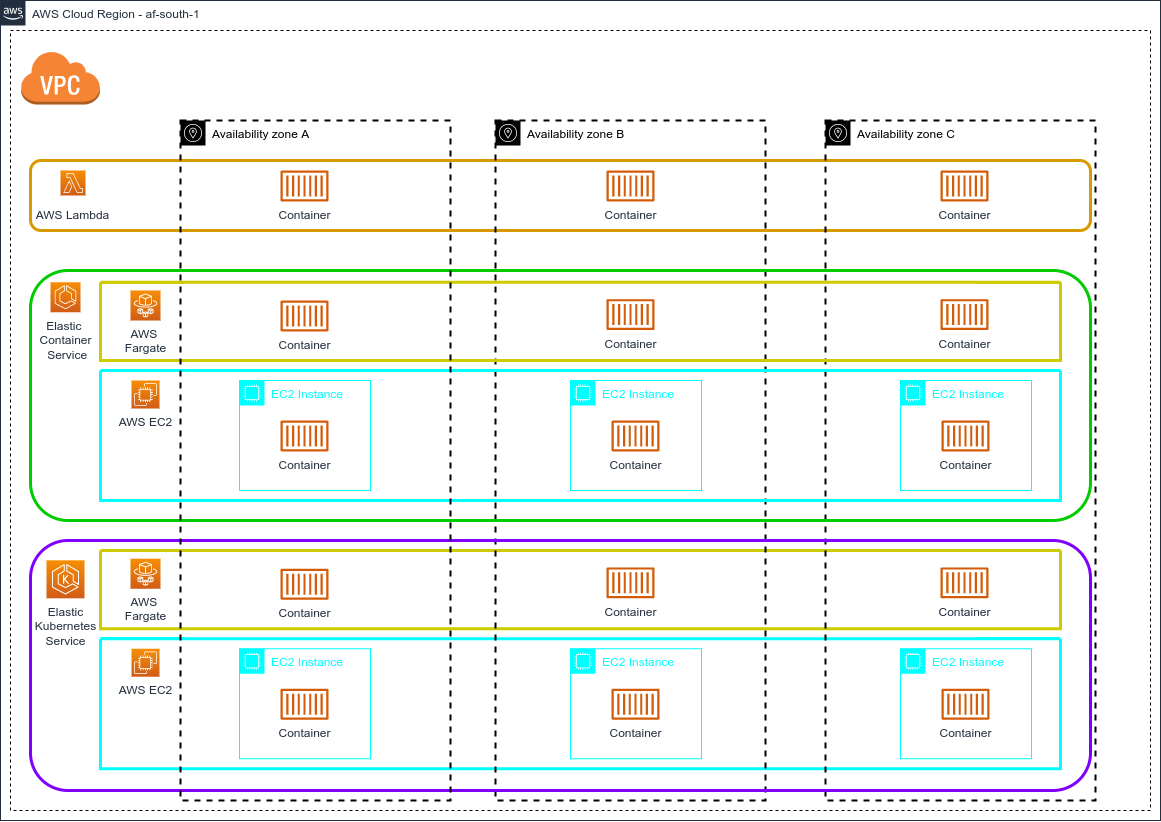
\includegraphics[keepaspectratio,width=\textwidth,height=\textheight]{archDiagram}
      \end{columns}
    
\end{frame}

% Full-size image
\fullimage{archDiagram}


% Title and text
\begin{frame}
  \Frametitle{Title and text}

  Here is some text.  \\[2ex] % vertical spacing

  \begin{enumerate}
    \item First
    \item Second
    \item Third
  \end{enumerate}
  
\end{frame}